% Compile with latex to get .div output
% Then execute dvisvgm to convert .div to .svg, use --no-fonts if fonts go wrong.
\documentclass[tikz]{standalone}
\usetikzlibrary{arrows.meta,positioning,automata}
\begin{document}
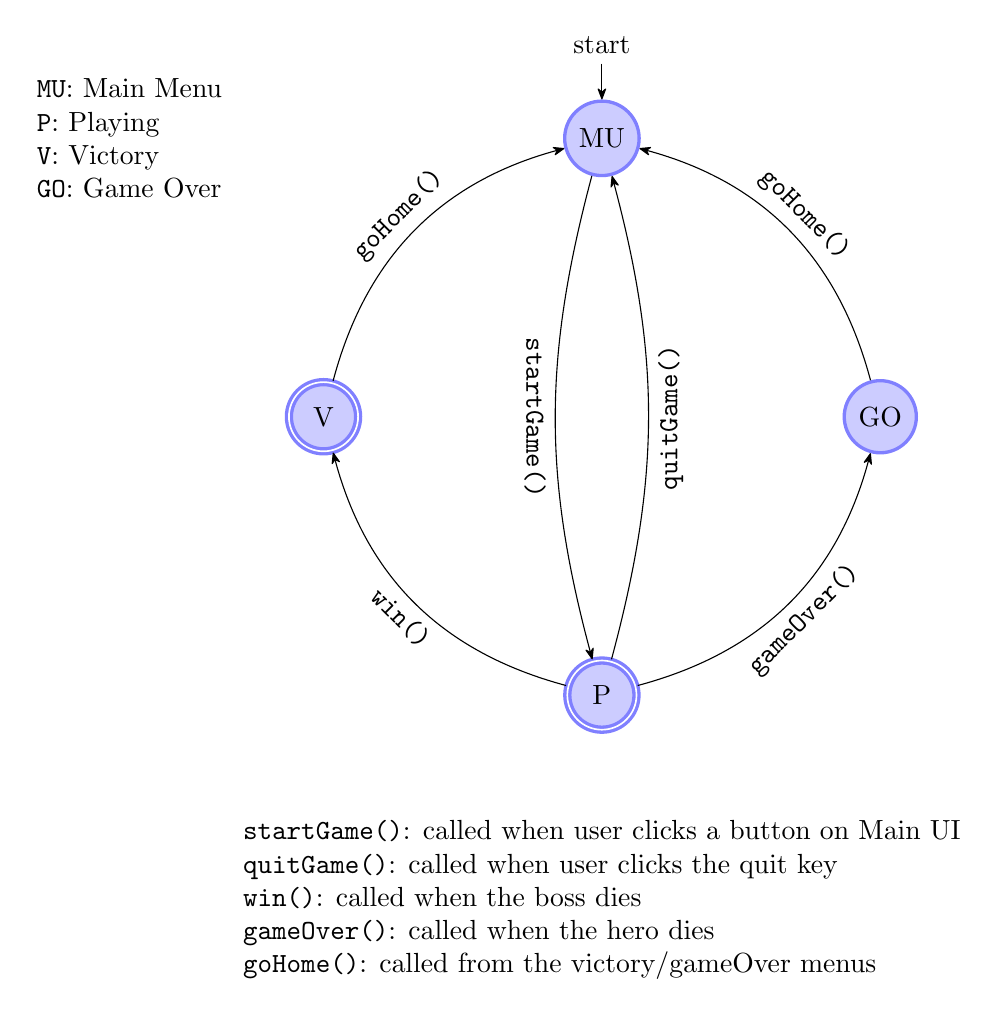
\begin{tikzpicture}[%
	node distance=5cm,on grid,>={Stealth[round]},
	every state/.style={draw=blue!50,very thick,fill=blue!20},
	initial where=above]
	
	\node (TXT) [align=left] {%
		\texttt{MU}: Main Menu\\
		\texttt{P}: Playing\\
		\texttt{V}: Victory\\
		\texttt{GO}: Game Over
	};

	\node[state,initial]	(MU)	[right=6cm of TXT]	{MU};
	\node[state,accepting]	(V)		[below left=of MU]	{V};
	\node[state]			(GO)	[below right=of MU]	{GO};
	\node[state,accepting]	(P)		[below right=of V]	{P};


	\path[->] (MU) edge	[bend right=15]	node	[sloped,below]	{\texttt{startGame()}}	
		(P);
	\path[->] (P) edge	[bend right=15]	node	[sloped,below]	{\texttt{quitGame()}}	
		(MU);
	\path[->] (P)  edge [bend right]	node	[sloped,below]	{\texttt{gameOver()}}
		(GO);
	\path[->] (P)  edge [bend left]		node	[sloped,below]	{\texttt{win()}}
		(V);
	\path[->] (V)  edge [bend left]		node	[sloped,above]	{\texttt{goHome()}}
		(MU);
	\path[->] (GO)  edge [bend right]	node	[sloped,above]	{\texttt{goHome()}}
		(MU);

	\node [anchor=north,below=1cm of P.south,align=left] {%
		\texttt{startGame()}: called when user clicks a button on Main UI\\
		\texttt{quitGame()}: called when user clicks the quit key\\
		\texttt{win()}: called when the boss dies\\
		\texttt{gameOver()}: called when the hero dies\\
		\texttt{goHome()}: called from the victory/gameOver menus
	};

\end{tikzpicture}
\end{document}